% !TEX root = ../thesis.tex

\chapter{模态不匹配2D-Markov跳变系统的异步滑模控制}
	在实际应用中,信息的传递可能会沿着多个维度传递,这样的系统我们称之为多维控制系统。当系统信息的传递方向只有两个的时候,我们称这样的多维系统为二维(2D)控制系统。2D控制系统的历史可以追溯到上个世纪70年代,现在已经被用来处理各种各样的实际应用,例如数字图像处理、偏微分方程建模和信号滤波\cite{roesser1975discrete,marszalek1984two,rogers2015multidimensional}等。同一维(1D)系统不同的是,二维系统的信息会沿着两个不同的方向传递,并且这两个方向的信息会相互作用,这意味着2D系统相对1D系统更加复杂,分析起来也更加困难。 为了描述2D系统的特殊结构和性质,学者们提出了一些基于状态空间的数学模型,其中比较流行的是Roesser模型 \cite{roesser1975discrete} 和 Fornasini-Marchesini 模型 \cite{fornasini1978doubly}。在Roesser模型中,系统状态由水平状态和垂直状态这两个独立的子状态组成,可以从当前状态分别推导出不同方向上的下一个水平状态和垂直状态。 与Roesser模型不同,Fornasini-Marchesini模型中的系统状态并不区分水平、垂直子状态,而是用一个向量来表示两个方向的信息,即该向量是具有两个独立变量的函数,并且当前系统状态是从它的左边相邻、下方相邻状态得到的。 在大多数情况下,Roesser模型可以看作是Fornasini-Marchesini模型的特例,但Rosser模型的表达形式更加直观,更容易理解,在某些情况下更便于系统分析。Du等人在文献\cite{du2001h,du2002hinfinity}中利用2D有界实引理建立了2D系统的$H_\infty$控制理论。随后,一些学者将这个成果推广到了具有时变延迟\cite{trinh2016stability}、多类噪声\cite{ahn2016stochastic}、不确定模态转移参数 \cite{chesi2016robust}等2D系统的控制、滤波问题中。Anh在文献\cite{ahn2015two}中,利用矩阵线性不等式方法研究了2D-Makrov跳变系统的无源控制和滤波问题。
	
	另一方面,滑模控制(SMC)是一种非常有效的控制技术。由于它对参数变化、外部干扰和不确定模型具有强大的鲁棒性,已成功应用于各种实际系统中\cite{utkin2009sliding,yang1999sliding,shima2006sliding}。滑模控制的主要思想是,首先构造一个滑模面,然后根据这个滑模面设计一个不连续的控制率,在该控制率的作用下,系统状态会不断的向滑模面靠近,最终达到滑模面或者进入到滑模面的某个领域内\cite{edwards1998sliding}。近年来,学者们对滑模控制进行了深入的研究,并针对Markov跳变系统取得了一系列重要的成果\cite{li2015state,wu2010state,wang2017smc}。一些学者对1D-Markov跳变系统模态不匹配的滑模控制问题进行了研究\cite{song2018asynchronous,li2017passivity,qi2018observer}。2D-Markov跳变系统同样吸引了一些学者的兴趣。如文献\cite{gao2004stabilization,wu2018hcontrol2d,wu2008hfiltering2d,wu2006modelreduction,shen2019dissipativity}分别对2D-Markov跳变系统的$H_\infty$控制、$H_\infty$滤波、$H_\infty$模型推导、故障检测等问题进行了讨论。但是到目前为止,尚且没有文章研究2D-Markov跳变系统的滑模控制问题。
	
	本章中,我们将研究2D-Markov跳变系统的滑模控制问题。考虑到2D系统的特殊结构和特性,我们将构造一个全新的2D滑模面。另一方面,考虑控制器模态同系统模态的不匹配问题,我们引入隐马尔可夫模型来设计滑模控制器。同时,我们将对系统的稳定性、$H_\infty$性能、系统状态到滑模面的可达性等问题分别展开讨论。

\section{数学模型及问题描述}
	本章考虑如下由Roesser模型描述2D-Markov跳变系统:
	\begin{equation} \label{system-equation}
	\left\{ 
	\begin{array}{lr}
	\begin{split}
	\emph{\textbf{x(i, j)}} = A_{r(i,j)}x(i,j)+B_{r(i,j)}[(u(i,j)+f(x(i,j),r(i,j))]+E_{r(i,j)}w(i,j),
	\end{split}\\
	\begin{split}
	y(i,j) = C_{r(i,j)}x(i,j)+D_{r(i,j)}w(i,j),
	\end{split}
	\end{array}
	\right.
	\end{equation}
	其中,
	\begin{equation*}
	\emph{\textbf{x(i, j)}} = \begin{bmatrix}
	x^{h}(i+1,j)\\
	x^{v}(i,j+1)
	\end{bmatrix}, \ 
	x(i, j) = \begin{bmatrix}
	x^{h}(i,j)\\
	x^{v}(i,j)
	\end{bmatrix}          
	\end{equation*}
	这里,	$x^{h}(i,j)\in \mathbb{R}^{n_h}$, $x^{v}(i,j)\in \mathbb{R}^{n_v}$ 分别表示水平、垂直两个方向的子系统状态, $u(i,j) \in \mathbb{R}^{n_u}$,$y(i,j) \in \mathbb{R}^{n_y}$ 分别表示控制输入和被控输出, 以及 $w(i,j) \in \mathbb{R}^{n_w}$ 表示外部扰动,并满足条件$\ell_{2}\{[0,\infty),[0,\infty)\}$。 $A_{r(i,j)}$, $B_{r(i,j)}$, $C_{r(i,j)}$, $D_{r(i,j)}$ 及 $E_{r(i,j)}$ 表示已知具有合适维度的系统时变矩阵。 同时,我们假设对任意的 $r(i,j)\in\mathcal{N}_{1}$,矩阵$B_{r(i,j)}$是列满秩的,即rank($B_{r(i,j)}$)$=n_u$。 非线性函数 $f(x(i,j),r(i,j))$ 满足
	\begin{equation}\label{nonlinear-func}
	\|f(x(i,j),r(i,j)\| \leq \delta_{r(i,j)}\|x(i,j)\|
	\end{equation}
	其中, $\delta_{r(i,j)}$ 是一个已知的标量, $\|\cdot\|$ 表示欧拉范数。 参数 $r(i,j)$ 在集合 $\mathcal{N}_{1}=\{1,2...,N_{1} \}$ 中取值,同时满足模态转移矩阵 $\varLambda = [\lambda_{kp}]$,其对应的模态转移概率为  (参考文献\cite{wu2018hcontrol2d,wu2008hfiltering2d})
	\begin{equation}\label{tps_system}
	\begin{split}
	&\Pr\{r(i+1,j)=p|r(i,j)=k\}\\
	=&\Pr\{r(i,j+1)=p|r(i,j)=k\}=\lambda_{kp},\  \forall k,p \in \mathcal{N}_{1}
	\end{split}
	\end{equation}	
	这里,对任意的  $k, p\in\mathcal{N}_{1}$, $\lambda_{kp}\in[0,1]$,且对任意的 $k$,有$\sum_{p=1}^{N_1}\lambda_{kp}=1$。
	
	{\bf 注 \ \ 3.1:}
	注意到,条件\eqref{tps_system} 包含了一个隐含的假设,即系统模态沿着水平、垂直方向的跳变概率是一样的。
	
	下面我们对2D系统\eqref{system-equation}的初始条件 ($X_{0},\varGamma_{0}$) 做以下假设
	\begin{equation} \label{boundary-condition}
	\left\{
	\begin{array}{lr}
	\begin{split}
	X_{0} &= \{x^{h}(0,j),x^{v}(i,0)|\ i,j = 0,1,2...\}\\
	\varGamma_{0} &= \{r(0,j), r(i,0)|\ i,j = 0,1,2... \}
	\end{split}
	\end{array}
	\right.
	\end{equation}
	
	系统状态的零初始条件$X_0$设置为,对任意非负整数$i,j$,$x^{h}(0,j) =0, x^{v}(i,0)=0$。此外,对$X_{0}$施加如下假设
	
	{\bf 假设 \ \ 3.1:}
	边界条件$X_{0}$满足
	\begin{equation}
	\lim\limits_{Z\to\infty}\mathbb{E}\Big\{\sum_{z=1}^{Z}(\|x^{h}(0,z)\|^{2}+ \|x^{v}(z,0)\|^{2})\Big\} < \infty
	\end{equation}
	其中,$\mathbb{E}\{\cdot\}$表示数学期望。
	
	在实际控制系统中,控制器往往不能获得系统模态$r(i,j)$的全部信息。因此,在本章中,我们采用了隐Markov模型$(r(i,j),\sigma(i,j),\varLambda,\varPsi)$来描述控制器模态和系统模态之间存在的不匹配现象。这里,我们使用$\sigma(i,j)$来表示控制器模态,它在另一个集合$\mathcal{N}_{2} = \{1,2...N_{2}\}$中取值,且满足条件模态转移矩阵$\varPsi=[\mu_{k\tau} ]$,该矩阵对应的条件模态转移概率为
	\begin{equation}
	\Pr\{\sigma(i,j)=\tau|r(i,j)=k\}=\mu_{k\tau } %\forall  k\in\mathcal{N}_{1}, \tau\in\mathcal{N}_{2}
	\end{equation}
	这里,对任意的$k\in\mathcal{N}_{1}$,$\tau\in\mathcal{N}_{2}$, 有$\mu_{k\tau }\in[0,1]$,且对任意的模态$k$,有 $\sum_{\tau =1}^{N_{2}}\mu_{k\tau } = 1$ 。
	
	{\bf 注 \ \ 3.2:}
	隐Markov模型是一个包含了同步、异步及模态独立情况的综合模型。控制器属于哪种情况可由条件模态转移概率矩阵$\varPsi$来决定。当$\varPsi=\varLambda$时,控制器变成了一个模态同步控制器,当$\mathcal{N}_{2}=\{1\}$时,控制器变成了一个只包含一个模态的模态独立控制器。因此,我们得到的结果可以通过调节矩阵$\varPsi$,很容易推广到同步和模态独立的情况。
	
	下面,我们分别给出系统渐进均方稳定和 $H_{\infty}$ 性能的定义。	
	
	{\bf 定义 \ \ 3.1:}
	当$w(i,j)\equiv0$时, 如果下式对任意的初始条件$X_{0}$成立
	\begin{equation}\label{AMSS}
	\lim\limits_{i+j\to\infty}\mathbb{E}\{\|x(i,j)\|^{2}\} = 0
	\end{equation}
	我们称,在假设3.1意义下的2D-Markov跳变系统 \eqref{system-equation}是渐进均方稳定的。
	
	{\bf 定义 \ \ 3.2:}
	给定标量 $\gamma>0$,如果条件 \eqref{AMSS}及下面的公式在$w(i,j)\in\ell_{2}\{[0,\infty),[0,\infty)\}$时成立,
	\begin{equation} \label{invDef2}
	\sum_{i=0}^{\infty}\sum_{j=0}^{\infty}\mathbb\{\|y(i,j)\|^{2}\} <  \gamma^{2} \sum_{i=0}^{\infty}\sum_{j=0}^{\infty}\mathbb\{\|w(i,j)\|^{2}\}
	\end{equation}
	我们称,在零初始条件下的2D-Markov跳变系统\eqref{system-equation}是渐进均方稳定的,同时满足$H_{\infty}$性能$\gamma$。

	为了方便后续的推导,我们这里做一些符号简化。我们使用$k$来表示参数$r(i,j)$,使用$\tau$来表示$\sigma(i,j)$ 。

	本章的目的是,基于隐Markov模型,设计一个二维异步控制器,使得对应的Markov跳变系统是随机稳定的,并满足一定的$H_{\infty}$性能。
	
\section{主要成果}
	在本节,我们首先根据2D系统的结构特征,构造一个新颖的2D滑模面,同时基于隐Markov模型设计出对应的2D滑模控制器。之后,我们会分析系统的渐进均方稳定性,$H_{\infty}$性能,以及系统状态到滑模面的可达性。

\subsection{滑模面构造及异步2D滑模控制器设计} \label{sliding-surface}
	在本章中,我们根据2D系统的特性构造如下滑模面
	\begin{equation}\label{siding-surface-equation}	
	s(i,j) = \begin{bmatrix}
	s^{h}(i,j)\\
	s^{v}(i,j)
	\end{bmatrix}
	= Gx(i,j)
	\end{equation}
	这里,$s^{h}(i,j)$、 $s^{v}(i,j)$分别代表水平、垂直方向的子滑模面,矩阵$G=\sum_{k=1}^{N_{1}}\beta_{k}B^{T}_{k}$。 这里需要注意的是,我们应该选择合适的 $\beta_{k}$ 使得矩阵$GB_{k}$ 对任意的$k\in\mathcal{N}_{1}$都是非齐次的。 根据假设 $B_{k}$ 对任意的$k\in\mathcal{N}_{1}$是列满秩的, 因此只要选择合适的 $\beta_{k}$就一定可以使得上述要求得以满足。 
	
	考虑到控制器模态同系统模态的不匹配问题,设计如下的异步2D滑模控制器
	\begin{equation}\label{smc-law}
	u(i,j) = K_{\tau }x(i,j)-\rho(i,j)\frac{s(i,j)}{\|s(i,j)\|}
	\end{equation}
	这里,矩阵$K_{\tau }\in\mathbb{R}^{n_u\times n_x}$是待确定的控制器增益, 且满足 $n_x=n_h+n_v$, 参数 $\rho(i,j)$ 设定为
	\begin{equation}\label{varrho}
	\rho(i,j) = \varrho_{1}\|x(i,j)\| + \varrho_{2}\|w(i,j)\|
	\end{equation}
	其中, $\varrho_{1}=\max_{k\in\mathcal{N}_{1}} \{\delta_{k} \}$, $\varrho_{2} = \max_{k\in\mathcal{N}_{1}}\{\|(GB_{k})^{-1}GE_{k}\| \} $, 参数 $\delta_{k}$ 在条件\eqref{nonlinear-func}中已经给出。 
	
	由系统方程\eqref{system-equation}及异步2D控制器\eqref{smc-law},我们可以得到如下闭环2D-Markov跳变系统
	\begin{equation} \label{closed-loop-system-equation}
	\emph{\textbf{x(i, j)}} = \bar{A}_{k\tau }x(i,j)+B_{k}\bar{\rho}_{k}(i,j)+E_{k}w(i,j)
	\end{equation}
	其中, $\bar{A}_{k\tau } = A_{k}+B_{k}K_{\tau }$,$\bar{\rho}_{k}(i,j)$ 为
	\begin{equation*}
	\bar\rho_{k}(i,j)=f_{k}(x(i,j))-\big(\varrho_{1}\|x(i,j)\|+\varrho_{2}\|w(i,j)\|\big)\cdot\frac{s(i,j)}{\|s(i,j)\|}.
	\end{equation*}
	下面,根据 \eqref{nonlinear-func} 及向量范数的性质, 我们可以推出
	\begin{equation}\label{norm-rho-inequality}
	\|\bar{\rho}_{k}(i,j)\| \leq (\varrho_{1}+\delta_{k})\|x(i,j)\| + \varrho_{2}\|w(i,j)\| ,
	\end{equation} 
	进一步可以得到
	\begin{equation}\label{rholeseq}
	\|\bar{\rho}_{k}(i,j)\|^{2} \leq 2(\varrho_{1}+\delta_{k})^{2}\|x(i,j)\|^{2} +2\varrho_{2}^{2}\|w(i,j\|^{2} .
	\end{equation}	
	
	{\bf 注 \ \ 3.3:}
	本文设计的控制器基于隐Markov模型 $(r(i,j),\sigma(i,j),\varLambda,\varPsi)$,在这个模型下,系统的模态由Markov过程$\{r(i,j), i,j=1,2\ \dots\}$控制,而控制器的模态则由条件转移概率$u_{k\tau}$得到,条件模态转移概率矩阵$\varPsi$建立了系统模态和控制器模态之间的联系,相比模态独立控制器更充分的利用了系统的模态信息,这是异步控制器相比模态独立控制器的一个优势。
	
	{\bf 注 \ \ 3.4:}
	正如在前文中所介绍的,1D滑模控问题已经获得了广泛的研究,比如文献\cite{song2018asynchronous,li2017passivity,qi2018observer}等。但是值得注意的是,2D滑模控制(不仅仅是异步控制)问题目前还没有人进行研究。实际上,2D系统的特殊性质给系统分析带来了更大的复杂性,1D系统得到的诸多结论不能直接的推广到2D系统中来,2D系统的滑模控制问题相对1D系统更加的复杂。因此我们需要从2D系统的结构出发,来研究2D系统的滑模控制问题。在本章中,我们基于Roesser模型的2D系统特性,重新的设计了一个二维滑模面$s(i,j)$,由于2D滑模控制率包含了 $x(i,j)$ 、$s(i,j)$,因此我们称所设计的滑模控制器是2D滑模控制器。

\subsection{稳定性及 $H_{\infty}$ 性能分析 } \label{stability&H_infty}	
	在本小节,我们将关注闭环2D-Markov跳变系统\eqref{closed-loop-system-equation}的稳定性及$H_{\infty}$ 性能分析。我们将会提出一个充分条件,使得系统渐进均方稳定,且满足一个$H_{\infty}$ 性能 $\gamma$。
	
	{\bf 定理 \ \ 3.1:}
	考虑满足假设3.1,在2D异步滑模控制率\eqref{smc-law}作用下的2D控制系统\eqref{system-equation}。 对任意的$k\in\mathcal{N}_{1}, \tau\in\mathcal{N}_{2}$,给定标量 $\gamma>0$,如果存在矩阵 $K_{\tau }\in\mathbb{R}^{n_u\times n_x}$,  $R_{k}=\mathrm{diag}\{R^{h}_{k},R^{v}_{k}\}>0$,  $Q_{k\tau }>0$, $T_{k\tau }>0$ ,标量$\epsilon_{k}>0$, 有下列不等式成立
	\begin{equation}\label{T1C1}
	B^{T}_{k}  	\mathcal{R}_{k} B_{k} -\epsilon_{k}I \leq 0
	\end{equation}
	\begin{equation}\label{T1C2}
	\mathcal{A} +2\Big(\sum_{\tau =1}^{N_{2}}\mu_{k\tau } \mathrm{diag}\{Q_{k\tau }, T_{k\tau }\}\Big) < 0
	\end{equation}
	\begin{equation}\label{T1C3}
	\hat{A}^{T}_{k\tau }\mathcal{R}_{k}\hat{A}_{k\tau } - \mathrm{diag}\{Q_{k\tau }, T_{k\tau }\} < 0
	\end{equation}
	其中,
	\begin{equation*}
	\mathcal{A}=\begin{bmatrix}
	\varPi_{1} & \varPi_{3}\\
	*&\varPi_{2}
	\end{bmatrix}
	\end{equation*} 且,
	\begin{equation*} \label{varPi}
	\left\{
	\begin{array}{lr}
	\begin{split}
	\varPi_{1}&=-R_{k}+4(\delta_{k}+\varrho_{1})^{2}\epsilon_{k}I+C^{T}_{k}C_{k}\\
	\varPi_{2}&=-\gamma^{2}I+D^{T}_{k}D_{k}+4\varrho_{2}^{2}\epsilon_{k}I\\
	\varPi_{3}&= C_{k}^{T}D_{k}\\
	\end{split}
	\end{array}
	\right.
	\end{equation*}
	这里,$\mathcal{R}_{k}=\sum_{p=1}^{N1}\lambda_{kp}R_{p}$, $\hat{A}_{k\tau }=\begin{bmatrix}
	\bar{A}_{k\tau }& E_{k}
	\end{bmatrix}$。
	那么,我们称闭环2D-Markov跳变系统\eqref{closed-loop-system-equation} 是渐进均方稳定的,且满足 $H_{\infty}$性能$\gamma$。
	
	{\bf 证明:} 
	我们首先来研究系统的稳定性问题。 选择李雅普诺夫函数为 $V_{1}(i,j) = x^{T}(i,j)R_{r(i,j)}x(i,j)$,并定义
	\begin{equation}\label{VAR-DELTA-V1}
	\begin{split}
	\varDelta V_{1}(i,j) = \emph{\textbf{x(i, j)}}^{T} R^{*}(i,j) \emph{\textbf{x(i, j)}} - x^{T}(i,j)R_{k}x(i,j)
	\end{split}
	\end{equation}
	这里,$R^{*}(i,j)=\mathrm{diag}\{R^{h}_{r(i+1,j)},R^{v}_{r(i,j+1)}\}$。\\
	在$w(i,j)=0$时,由闭环控制系统 \eqref{closed-loop-system-equation},我们可以得到 
	\begin{equation}
	\begin{split}
	\mathbb{E}\{\varDelta V_{1}(i,j) \}&=\mathbb{E}\{\emph{\textbf{x(i, j)}}^{T}\mathcal{R}_{k}\emph{\textbf{x(i, j)}} - x^{T}(i,j)R_{k}x(i,j) \} \\
	&=  \sum_{\tau =0}^{N_{2}}\mu_{k\tau }\Big\{\big[\bar{A}_{k\tau }x(i,j)+B_{k}\bar{\rho}_{k}(i,j)\big]^{T}\mathcal{R}_{k}\\
	&\times\big[\bar{A}_{k\tau }x(i,j)+B_{k}\bar{\rho}_{k}(i,j)\big]\Big\}\\
	&- x^{T}(i,j)R_{k}x(i,j) \\
	&\leq x^{T}(i,j) \Big\{2\big(\sum_{\tau =1}^{N_{2}}\mu_{k\tau }\bar{A}^{T}_{k\tau }(i,j)\mathcal{R}_{k}\bar{A}_{k\tau }\big)\Big\}x(i,j)\\ &+2\bar{\rho}^{T}_{k}(i,j)B^{T}_{k}\mathcal{R}_{k}B_{k}\bar{\rho}_{k}(i,j) \\
	&-  x^{T}(i,j)R_{k}x(i,j)
	\end{split}
	\end{equation}
	由条件\eqref{norm-rho-inequality} 、\eqref{T1C1},可以推出
	\begin{equation}\label{combine-one-1}
	\begin{split}
	\mathbb{E}\{\varDelta  V_{1}(i,j) \} \leq x^{T}(i,j)\mathcal{G}_{k\tau }x(i,j)
	\end{split}
	\end{equation}
	其中, $\mathcal{G}_{k\tau }= 2\big(\sum_{\tau =1}^{N_{2}}\mu_{k\tau }\bar{A}^{T}_{k\tau }\mathcal{R}_{k}\bar{A}_{k\tau }\big)
	+ 2\epsilon_{k}(\delta_{k}+\varrho_{1})^{2}I- R_{k}$。
	根据正定矩阵的性质,可以由 \eqref{T1C2} ) 推出
	\begin{equation}
	2\big(\sum_{\tau =1}^{N_{2}}\mu_{k\tau }Q_{k\tau }\big)+4\epsilon_{k}(\delta_{k}+\varrho_{1})^{2}I+C^{T}_{k}C_{k}-R_{k} < 0
	\end{equation}
	进一步可以得到
	\begin{equation}\label{combine-one-2}
	2\big(\sum_{\tau =1}^{N_{2}}\mu_{k\tau }Q_{k\tau }\big)+2\epsilon_{k}(\delta_{k}+\varrho_{1})^{2}I-R_{k} < 0
	\end{equation}
	由条件 \eqref{T1C3}可以得到 
	\begin{equation}\label{combine-one-3}
	\bar{A}^{T}_{k\tau }\mathcal{R}_{k}\bar{A}_{k\tau }-Q_{k\tau } < 0
	\end{equation}
	由\eqref{combine-one-2}、\eqref{combine-one-3} 可以发现 $\mathcal{G}_{k\tau }<0$, 等价于
	\begin{equation}
	\mathcal{G}_{k\tau } \leq -\alpha I
	\end{equation}
	这里 $\alpha>0$。
	根据 \eqref{combine-one-1} 我们可以进一步得到
	\begin{equation}\label{VleqAlpha}
	\mathbb{E}\{\varDelta V_{1}(i,j) \} \leq-\alpha \mathbb{E}\{\|x(i,j)\|^{2} \}
	\end{equation}
	对上式累加\eqref{VleqAlpha}推出
	\begin{equation} \label{levE}
	\mathbb{E}\Big\{\sum_{i=0}^{\hat{\kappa}_{1}}\sum_{j=0}^{\hat{\kappa}_{2}}  \|x(i,j)\|^{2} \Big\} \leq -\frac{1}{\alpha} \mathbb{E}\Big\{\sum_{i=0}^{\hat{\kappa}_{1}}\sum_{j=0}^{\hat{\kappa}_{2}}  \varDelta V_{1}(i,j)  \Big\}
	\end{equation}
	这里 $\hat{\kappa}_{1}$, $\hat{\kappa}_{2}$ 是任意的正整数。 用 \eqref{VAR-DELTA-V1} 来代替 $\varDelta V_{1}$,同时,令 $R_{k}=\mathrm{diag}\{R^{\rm{h}}_{k},R^{\rm{v}}_{k}\}$ (见定理3.1) ,可以推出
	\begin{equation} \label{Vhv}
	\begin{split}
	&\sum_{i=0}^{\hat{\kappa}_{1}}\sum_{j=0}^{\hat{\kappa}_{2}}  \varDelta V_{1}(i,j)\\&= \sum_{i=0}^{\hat{\kappa}_{1}}\big\{V^{v}_{1}(i,\hat{\kappa}_{2}+1) - V^{v}_{1}(i,0) \big\}+  \sum_{j=0}^{\hat{\kappa}_{2}}\big\{V^{h}_{1}(\hat{\kappa}_{1}+1,j) - V^{h}_{1}(0,j) \big\}\\
	&\leq -\big( \sum_{i=0}^{\hat{\kappa}_{1}}V^{v}_{1}(i,0) + \sum_{j=0}^{\hat{\kappa}_{2}}V^{h}_{1}(0,j)\big) \\
	%			&\leq -\beta \sum_{\ell=0}^{\infty} \big(  \|x^{v}(\ell,0)\|^{2} + \|x^{h}(0,\ell)\|^{2} \big)
	\end{split}
	\end{equation} 
	这里,我们定义$V_{1}^{h}(i,j)$ 和 $V_{1}^{v}(i,j)$ 如下  
	\begin{equation*}
	\left\{
	\begin{array}{lr}
	\begin{split}
	V^{h}_{1}(i,j)=x^{hT}(i,j)R^{h}_{r(i,j)}x^{h}(i,j)\\
	V^{v}_{1}(i,j)=x^{vT}(i,j)R^{v}_{r(i,j)}x^{v}(i,j)
	\end{split}
	\end{array}
	\right.
	\end{equation*}
	根据边界条件假设3.1,同时令$\hat{\kappa}_{1}$, $\hat{\kappa}_{2}$ 趋向无穷, 由\eqref{levE} 及\eqref{Vhv} 可以推出
	\begin{equation}
	\begin{split}
	\mathbb{E}\Big\{\sum_{i=0}^{\hat{\kappa}_{1}}\sum_{j=0}^{\hat{\kappa}_{2}}  \|x(i,j)\|^{2} \Big\} &\leq \frac{\beta}{\alpha} \sum_{\ell=0}^{\infty} \big(  \|x^{v}(\ell,0)\|^{2} + \|x^{h}(0,\ell)\|^{2} \big)<\infty
	\end{split}	
	\end{equation}
	这里 $\beta$ (显然,$\beta>0$) 是对任意的$\ell=0,1,2...$,$R^{h}_{r(0,\ell)}$ 和 $R^{v}_{r(\ell,0)}$的最大特征值。上式意味着 \eqref{AMSS} 成立。至此,我们证明了闭环控制系统是渐进均方稳定的。
	
	下面我们来研究在零初始条件下系统的$H_{\infty}$性能问题。 根据闭环控制系统\eqref{closed-loop-system-equation},不难推出
	\begin{equation}\label{DETAV1}
	\begin{split}
	\mathbb{E}\{\varDelta V_{1}(i,j) \} &=  \sum_{\tau =0}^{N_{2}}\mu_{k\tau }\Big\{\big[\bar{A}_{k\tau }x(i,j)+B_{k}\bar{\rho}_{k}(i,j)+E_{k}w(i,j)\big]^{T}\\
	&\times \mathcal{R}_{k}\big[\bar{A}_{k\tau }x(i,j)+B_{k}\bar{\rho}_{k}(i,j)+E_{k}w(i,j)\big]\Big\}\\
	&- x^{T}(i,j)R_{k}x(i,j) \\
	&\leq \hat{x}^{T}(i,j) \Big\{2\big(\sum_{\tau =1}^{N_{2}}\mu_{k\tau }\hat{A}^{T}_{k\tau }(i,j)\mathcal{R}_{k}\hat{A}_{k\tau }\big)\Big\}\hat{x}(i,j)\\ &+2\bar{\rho}^{T}_{k}(i,j)B^{T}_{k}\mathcal{R}_{k}B_{k}\bar{\rho}_{k}(i,j) \\
	&-  x^{T}(i,j)R_{k}x(i,j)\\
	\end{split}
	\end{equation}
	%	where $\hat{x}(i,j)=\begin{bmatrix}
	%		x(i,j)\\ w(i,j)
	%	\end{bmatrix}$, $\hat{A}_{k\tau }(i,j)=\begin{bmatrix}
	%		\bar{A}_{k\tau }&E_{k}
	%	\end{bmatrix}$.
	这里
	\begin{equation*}
	\hat{x}(i,j)=\begin{bmatrix}
	x(i,j)\\ w(i,j)
	\end{bmatrix},\ \hat{A}_{k\tau }(i,j)=\begin{bmatrix}
	\bar{A}_{k\tau }&E_{k}
	\end{bmatrix}
	\end{equation*}
	注意到条件 \eqref{rholeseq} 及\eqref{T1C1},可以推出
	\begin{equation}\label{invRho}
	\begin{split}
	&\bar{\rho}^{T}_{k}(i,j)B^{T}_{k}\mathcal{R}_{k}B_{k}\bar{\rho}_{k}(i,j)\\
	&\leq \|B^{T}_{k}\mathcal{R}_{k}B_{k}\|\|\bar{\rho}_{k}\|^{2} \\
	&\leq 2\epsilon_{k}\big((\delta_{k}+\varrho_{1})^{2}\|x(i,j)\|^{2}+\varrho_{2}^{2}\|w(i,j)\|^{2} \big)
	\end{split}
	\end{equation} 
	由条件 \eqref{T1C2} 及 \eqref{T1C3}可以得到下式
	\begin{equation}\label{T1P4}
	\mathcal{\varXi}_{k\tau }<0
	\end{equation}	
	其中, $\mathcal{\varXi}_{k\tau } \equiv \mathcal{A} +2\sum_{\tau =1}^{N_{2}}\mu_{k\tau }\hat{A}^{T}_{k\tau }\mathcal{R}_{k}\hat{A}_{k\tau }$。
	由系统方程 \eqref{system-equation},且把\eqref{invRho} 带入 \eqref{DETAV1} 可以得到
	\begin{equation}\label{DETAV1ZW}
	\begin{split}
	\mathbb{E}\{\varDelta V_{1}(i,j)+\|y(i,j)\|^{2}-\gamma^{2}\|w(i,j)\|^{2}  \} \leq \hat{x}^{T}(i,j)\mathcal{\varXi}_{k\tau } \hat{x}(i,j)<0
	\end{split}
	\end{equation}
	注意到在零初始条件下的\eqref{Vhv} 我们可以推出
	\begin{equation} \label{Vhv2}
	\begin{split}
	&\sum_{i=0}^{\hat{\kappa}_{1}}\sum_{j=0}^{\hat{\kappa}_{2}}  \varDelta V_{1}(i,j)\\
	&=\sum_{i=0}^{\hat{\kappa_{1}}}V^{v}_{1}(i,\hat{\kappa}_{2}+1) + \sum_{j=0}^{\hat{\kappa}_{2}}V^{h}_{1}(\hat{\kappa}_{1}+1,j) \\
	&\geq 0 \qquad \forall \hat{\kappa}_{1},\hat{\kappa}_{2} = 1,2,3...
	\end{split}
	\end{equation}
	接下来,由 \eqref{DETAV1ZW} 和 \eqref{Vhv2} 我们可以得到 
	\begin{equation}\label{DETAV1ZW2}
	\begin{split}
	&\sum_{i=0}^{\infty}\sum_{j=0}^{\infty}  \mathbb{E}\{\|y(i,j)\|^{2}-\gamma^{2}\|w(i,j)\|^{2}  \}\\
	&\leq \sum_{i=0}^{\infty}\sum_{j=0}^{\infty}  \mathbb{E}\{\varDelta V_{1}(i,j)+\|y(i,j)\|^{2}-\gamma^{2}\|w(i,j)\|^{2}  \}  \\
	&< 0
	\end{split}
	\end{equation}
	进而 \eqref{invDef2}成立。 至此,我们完成了定理的证明。
	
\subsection{滑模面可达性分析}\label{minimization} 
	在本小节,我们将会分析在设计的异步控制率作用下的系统状态到所构造滑模面的可达性问题。借助Lyapunov方法,我们会提供一个充分条件,使得在异步滑模控制率\eqref{smc-law}可以迫使系统状态轨迹进入到一个预先设定的滑模域内部。
	
	{\bf 定理 \ \ 3.2:}
	考虑在异步2D滑模控制率作用下的闭环2D-Markov跳变系统\eqref{closed-loop-system-equation}。如果对任意的$k\in\mathcal{N}_{1}$,$\tau\in\mathcal{N}_{2}$,存在矩阵 $K_{\tau }\in\mathbb{R}^{n_u\times n_x}$, $R_{k}>0$, $F_{k}>0$,标量 $\epsilon_{k}>0$,  使得条件 \eqref{T1C1} 及下面的式子成立
	\begin{equation} \label{T2C1}
	2\sum_{\tau =1}^{N_{2}} \bar{A}^{T}_{k\tau }\big(\mathcal{R}_{k}+G^{T}\mathcal{F}_{k}G\big)\bar{A}_{k\tau }-R_{k} <0
	\end{equation}
	这里, $\mathcal{R}_{k}$ 在定理 3.1中定义了,且矩阵 $\mathcal{F}_{k}=\sum_{p=1}^{N_{1}}\lambda_{kp}F_{p}$。那么,闭环2D控制系统   \eqref{closed-loop-system-equation} 的系统状态将会进入一个滑模域 $\mathcal{O}$内,该滑模域围绕预先定义的滑模面 \eqref{siding-surface-equation},且定义为
	\begin{equation}\label{smc-region}
	\mathcal{O}\equiv\Big\{\|s(i,j)\|\leq\ \rho^{*}(i,j) \Big\}
	\end{equation} 
	这里$\rho^{*}(i,j) = \mathrm{max}_{k\in\mathcal{N}_{1}}\sqrt{\hat{\rho}_{k}(i,j)/
		\lambda_{\mathrm{min}}(F_{k})}$,其中
	\begin{equation*}
	\begin{split}
	\hat{\rho}_{k}(i,j)=&4\big(\|E^{T}_{k}\mathcal{R}_{k}E_{k}\|+ \|E^{T}_{k}G^{T}\mathcal{R}_{k}GE_{k}\|\\
	&+2\varrho_{2}^{2}(\|B^{T}_{k}\mathcal{F}_{k}B_{k}\|+ \|B^{T}_{k}G^{T}\mathcal{F}_{k}GB_{k}\| )\big)\|w(i,j)\|^{2}\\
	+&8(\varrho_{1}+\delta_{k})^{2}\big(\|B^{T}_{k}\mathcal{R}_{k}B_{k}\|+\|B^{T}_{k}G^{T}\mathcal{R}_{k}GB_{k}\|\big)\|x(i,j)\|^{2}.
	\end{split}
	\end{equation*}
	这里 $\lambda_{\mathrm{min}}(F_{k})$ 在此时表示矩阵 $F_{k}$的最小特征值。
	
	{\bf 证明:} 
	首先,我们定义$\emph{\textbf{s(i, j)}} = \begin{bmatrix}
	s^{h}(i+1,j)\\ s^{v}(i,j+1)
	\end{bmatrix}$,  显然$\emph{\textbf{s(i, j)}}=G\emph{\textbf{x(i, j)}}$。 然后我们选择如下李雅普诺夫函数
	\begin{equation}\label{LyapunoovT}
	V(i,j)=V_{1}(i,j)+V_{2}(i,j)
	\end{equation}
	这里 $V_{1}(i,j)$ 同定理3.1, $V_{2}(i,j)=s^{T}(i,j)F_{r(i,j)}s(i,j)$。 同定理3.1的证明过程相似,我们不难推出
	\begin{equation} \label{P2T1}
	\begin{split}
	&\mathbb{E}\{\varDelta V_{1}(i,j) \}\\
	&=\mathbb{E}\Big\{\emph{\textbf{x(i, j)}}^{T}R^{*}(i,j)\emph{\textbf{x(i, j)}} - x^{T}(i,j)R_{k}x(i,j)\Big\}\\
	&=  \sum_{\tau =0}^{N_{2}}\mu_{k\tau }\Big\{\big[\bar{A}_{k\tau }x(i,j)+B_{k}\bar{\rho}_{k}(i,j)+E_{k}w(i,j)\big]^{T}\\
	&\times\mathcal{R}_{k} \big[ \bar{A}_{k\tau }x(i,j)+B_{k}\bar{\rho}_{k}(i,j)+E_{k}w(i,j)\big]\Big\}\\
	&-x^{T}(i,j)R_{k}x(i,j)\\
	&\leq 2x^{T}(i,j)\sum_{\tau =1}^{N_{2}}\mu_{k\tau }\bar{A}^{T}_{k\tau }\mathcal{R}_{k}\bar{A}_{k\tau }x(i,j) \\
	&+2\big[B_{k}\bar{\rho}_{k}(i,j)+E_{k}w(i,j)\big]^{T}\mathcal{R}_{k} \big[B_{k}\bar{\rho}_{k}(i,j)+E_{k}w(i,j)\big]
	-x^{T}(i,j)R_{k}x(i,j)\\
	&\leq 2x^{T}(i,j)\sum_{\tau =1}^{N_{2}}\mu_{k\tau }\bar{A}^{T}_{k\tau }\mathcal{R}_{k}\bar{A}_{k\tau }x(i,j) 
	+ 4\bar{\rho}^{T}_{k}(i,j)B^{T}_{k}\mathcal{R}_{k}B_{k}\bar{\rho}_{k}(i,j)\\
	&+4w^{T}(i,j)E^{T}_{k}\mathcal{R}_{k}E_{k}w(i,j)
	-x^{T}(i,j)R_{k}x(i,j)
	%&\mathbb{E}\{\varDelta V_{1}(i,j) \}\\
	%=&\mathbb{E}\Big\{\emph{\textbf{x(i, j)}}^{T}R_{p}\emph{\textbf{x(i, j)}} - x^{T}(i,j)R_{k}x(i,j)\Big\}\\
	%=&  \sum_{\tau =0}^{N_{2}}\mu_{k\tau }\Big\{\big[\bar{A}_{k\tau }x(i,j)+B_{k}\bar{\rho}_{k}(i,j)+E_{k}w(i,j)\big]^{T}\\
	%\times&\mathcal{R}_{k} \big[ \bar{A}_{k\tau }x(i,j)+B_{k}\bar{\rho}_{k}(i,j)+E_{k}w(i,j)\big]\Big\}\\
	%-&x^{T}(i,j)R_{k}x(i,j)\\
	%\leq& 2x^{T}(i,j)\sum_{\tau =1}^{K_{2}}\mu_{k\tau }\bar{A}^{T}_{k\tau }\mathcal{R}_{k}\bar{A}_{k\tau }x(i,j) \\
	%+&2\big[B_{k}\bar{\rho}_{k}(i,j)+E_{k}w(i,j)\big]^{T}\mathcal{R}_{k}\\
	%\times&\big[B_{k}\bar{\rho}_{k}(i,j)+E_{k}w(i,j)\big]\\
	%-&x^{T}(i,j)R_{k}x(i,j)\\
	%\leq& 2x^{T}(i,j)\sum_{\tau =1}^{K_{2}}\mu_{k\tau }\bar{A}^{T}_{k\tau }\mathcal{R}_{k}\bar{A}_{k\tau }x(i,j) \\
	%+& \bar{\rho}^{T}_{k}(i,j)B^{T}_{k}\mathcal{R}_{k}B_{k}\bar{\rho}_{k}(i,j)\\
	%+&w^{T}(i,j)E^{T}_{k}\mathcal{R}_{k}E_{k}w(i,j)\\
	%-&x^{T}(i,j)R_{k}x(i,j)
	\end{split}
	\end{equation}
	这里 $R^{*}(i,j)$ 同定理3.1中定义。
	根据滑模面函数 \eqref{siding-surface-equation},我们可以推出
	\begin{equation} \label{P2T2}
	\begin{split}
	&\mathbb{E}\{\varDelta V_{2}(i,j) \}\\
	&=\mathbb{E}\Big\{\emph{\textbf{s(i, j)}}^{T}F^{*}(i,j)\emph{\textbf{s(i, j)}} - s^{T}(i,j)F_{k}s(i,j)\Big\}\\
	&=  \sum_{\tau =0}^{N_{2}}\mu_{k\tau }\Big\{\big[\bar{A}_{k\tau }x(i,j)+B_{k}\bar{\rho}_{k}(i,j)+E_{k}w(i,j)\big]^{T}\\ &\times G^{T}\mathcal{F}_{k} G\big[ \bar{A}_{k\tau }x(i,j)+B_{k}\bar{\rho}_{k}(i,j)+E_{k}w(i,j)\big]\Big\}\\
	&-s^{T}(i,j)F_{k}s(i,j)\\
	&\leq 2x^{T}(i,j)\sum_{\tau =1}^{N_{2}}\mu_{k\tau }\bar{A}^{T}_{k\tau }G^{T}\mathcal{F}_{k}G\bar{A}_{k\tau }x(i,j) \\
	&+2\big[B_{k}\bar{\rho}_{k}(i,j)+E_{k}w(i,j)\big]^{T}G^{T}\mathcal{F}_{k}  G\big[B_{k}\bar{\rho}_{k}(i,j)+E_{k}w(i,j)\big]\\
	&-s^{T}(i,j)F_{k}s(i,j)\\
	&\leq 2x^{T}(i,j)\sum_{\tau =1}^{N_{2}}\mu_{k\tau }\bar{A}^{T}_{k\tau }G^{T}\mathcal{F}_{k}G\bar{A}_{k\tau }x(i,j) 
	+ 4\bar{\rho}^{T}_{k}(i,j)B^{T}_{k}G^{T}\mathcal{F}_{k}GB_{k}\bar{\rho}_{k}(i,j)\\
	&+4w^{T}(i,j)E^{T}_{k}G^{T}\mathcal{F}_{k}GE_{k}w(i,j)
	-s^{T}(i,j)F_{k}s(i,j)
	\end{split}
	\end{equation}
	这里 $F^{*}(i,j)=\mathrm{diag}\{F^{h}_{r(i+1,j)},F^{v}_{r(i,j+1)}\}$。
	由条件 \eqref{LyapunoovT}-\eqref{P2T2},我们可以推出
	\begin{equation}\label{P2T3}
	\begin{split}
	&\mathbb{E}\{\varDelta V(i,j) \}\\
	&= \mathbb{E}\Big\{\varDelta_{1}(i,j)+\varDelta V_{2}(i,j) \Big\}\\
	&\leq x^{T}(i,j)\Big\{ 2\sum_{\tau =1}^{N_{2}}\mu_{k\tau }\bar{A}^{T}_{k\tau }\big(\mathcal{R}_{k} +G^{T}\mathcal{F}_{k}G\big)\bar{A}_{k\tau } \Big\} x(i,j) \\
	& +\vec{\rho}_{k}(i,j)-x^{T}(i,j)R_{k}x(i,j) - \lambda_{\mathrm{min}}(F_{k})\|s(i,j)\|^{2}\\
	\end{split}
	\end{equation}
	其中,
	\begin{equation*}
	\begin{split}
	&\vec{\rho}_{k}(i,j)\\
	&= 4\big(\|B^{T}_{k}\mathcal{F}_{k}B_{k}\|+ \|B^{T}_{k}G^{T}\mathcal{F}_{k}GB_{k}\|\big) \|\bar{\rho}_{k}(i,j)\|^{2} \\
	&+ 4\big(\|E^{T}_{k}\mathcal{R}_{k}E_{k}\|+ \|E^{T}_{k}G^{T}\mathcal{R}_{k}GE_{k}\|\big) \|w(i,j)\|^{2} 
	\end{split}
	\end{equation*}  
	显然,在用\eqref{rholeseq}替换 $\vec{\rho}_{k}(i,j)$后,我们可以推出,对任意的$k\in\mathcal{N}_{1}$, $\vec{\rho}_{k}(i,j) < \hat{\rho}_{k}(i,j)$。
	然后由条件 \eqref{T1C2}, 我们知道当系统状态在滑模域 $\mathcal{O}$外时有
	\begin{equation}\label{P2T5}
	-\lambda_{\mathrm{min}}(F_{k})\|s(i,j)\|^{2} + \vec{\rho}_{k}(i,j) <0
	\end{equation}
	由条件\eqref{T2C1}、 \eqref{P2T1}、 \eqref{P2T3} 、\eqref{P2T5} 可以得到
	\begin{equation}
	\begin{split}
	&\mathbb{E}\{\varDelta V(i,j) \} \leq x^{T}(i,j)\Big\{ 2\sum_{\tau =1}^{N_{2}}\mu_{k\tau }\bar{A}^{T}_{k\tau }\big(\mathcal{R}_{k} +G^{T}\mathcal{F}_{k}G \big)\bar{A}_{k\tau } -R_{k} \Big\} x(i,j)<0
	\end{split}
	\end{equation}
	也就是说,当系统状态在 $\mathcal{O}$外部时,  闭环控制系统\eqref{closed-loop-system-equation} 的状态轨迹将会严格的收敛到其内部。至此,证明完毕。
	
	
\subsection{异步2D滑模控制器综合分析 }\label{smc-law-synthesis} 
	显然,如果定理 3.1 和定理3.2同时成立的话, 我们就可以同时保证满足一定$H_{\infty}$的系统的随机稳定性及系统状态到滑膜面的可达性。下面,我们将会根据这个思路,继续我们的研究。
	
	{\bf 定理 \ \ 3.2:}
	考虑在假设3.1条件下,具有异步2D滑模控制器\eqref{smc-law}的控制系统 \eqref{system-equation}。给定标量$\gamma>0$,如果对任意的 $k\in\mathcal{N}_{1}, \tau\in\mathcal{N}_{2}$,存在矩阵 $\tilde{K}_{\tau }\in\mathbb{R}^{n_u\times n_x}$, $L_{\tau }\in\mathbb{R}^{n_x\times n_x}$, $\tilde{R}_{k}=\mathrm{diag}\{\tilde{R}^{h}_{k},\tilde{R}^{v}_{k}\}>0$, $\tilde{F}_{k}>0$,  $\tilde{Q}_{k\tau }>0$, $\tilde{T}_{k\tau }>0$ 及标量 $\tilde{\epsilon}_{k}>0$ 使得下面的条件成立
	\begin{equation} \label{T3C1}
	\begin{bmatrix}
	-\tilde{\epsilon}_{k}I &\mathscr{B}_{k}\\
	*& \mathscr{R}_{k}
	\end{bmatrix} < 0
	\end{equation}
	
	\begin{equation} \label{T3C2}
	\begin{bmatrix}
	\mathscr{L}_{k\tau }&\mathscr{A}_{k\tau }&\mathscr{G}_{k\tau }\\
	*&\mathscr{R}_{k}&0\\
	*&*&\mathscr{F}_{k}\\
	\end{bmatrix}<0
	\end{equation}
	
	\begin{equation}\label{T3C3}
	\begin{bmatrix}
	\mathscr{H}_{k}&\mathscr{D}_{k}&\mathscr{P}_{k\tau }&\mathscr{Y}_{k\tau }\\
	*&\mathscr{I}_{k}&0&0\\
	*&*&\mathscr{Q}_{k\tau }&0\\
	*&*&*&\mathscr{T}_{k\tau }\\
	\end{bmatrix} <0
	\end{equation}
	其中,
	\begin{equation}\notag
	\begin{split}
	\mathscr{B}_{k}&= \begin{bmatrix}
	\sqrt{\lambda_{k1}}\tilde{\epsilon}_{k}B^{T}_{k}&\sqrt{\lambda_{k2}}\tilde{\epsilon}_{k}B^{T}_{k}&\cdots&\sqrt{\lambda_{kN_{1}}}\tilde{\epsilon}_{k}B^{T}_{k}
	\end{bmatrix}\\
	\mathscr{R}_{k}&= \mathrm{diag}\{-\tilde{R}_{1}, -\tilde{R}_{2}, \cdots, -\tilde{R}_{N_{1}} \} \\
	\mathscr{F}_{k}&= \mathrm{diag}\{-\tilde{F}_{1}, -\tilde{F}_{2}, \cdots, -\tilde{F}_{N_{1}} \} \\	
	\mathscr{I}_{k} &= \mathrm{diag}\{-\tilde{\epsilon}_{k}, -I, -I, -\tilde{\epsilon}_{k} \}\\	
	\mathscr{Q}_{k\tau }&= \mathrm{diag}\{-\tilde{Q}_{k1}, -\tilde{Q}_{k2}, \cdots, -\tilde{Q}_{kN_{2}} \}\\
	\mathscr{T}_{k\tau }&= \mathrm{diag}\{-\tilde{T}_{k1}, -\tilde{T}_{k2}, \cdots, -\tilde{T}_{kN_{2}} \}\\
	\mathscr{L}_{k\tau }&= \mathrm{diag}\{\tilde{Q}_{k\tau }-L^{T}_{\tau }-L_{\tau },  -\tilde{T}_{k\tau } \}\\
	%			\begin{bmatrix}
	%				\tilde{Q}_{k\tau}-L^{T}_{\tau }-L_{\tau }&0\\
	%				*&-\tilde{T}_{k\tau }
	%			\end{bmatrix}, \
	\mathscr{H}_{k}\ &= \begin{bmatrix}
	-\tilde{R}_{k} & \tilde{R}C^{T}_{k}D^{T}_{k}\\
	*& -\gamma^{2}I
	\end{bmatrix} \\
	\mathscr{A}_{k\tau } &=\begin{bmatrix}
	\sqrt{\lambda_{k1}} \tilde{A}^{T}_{k\tau }& \cdots&\sqrt{\lambda_{kN_{1}}} \tilde{A}^{T}_{k\tau }\\
	\sqrt{\lambda_{k1}}\tilde{T}_{k\tau }B^{T}_{k} &\cdots&\sqrt{\lambda_{kN_{1}}} \tilde{T}_{k\tau }B^{T}_{k}\\
	\end{bmatrix} \\
	\mathscr{G}_{k\tau } &=\begin{bmatrix}
	\sqrt{\lambda_{k1}} \tilde{A}^{T}_{k\tau }G^{T}& \cdots&\sqrt{\lambda_{kN_{1}}} \tilde{A}^{T}_{k\tau }G^{T}\\
	0  &\cdots& 0
	\end{bmatrix}\\
	\mathscr{D}_{k\tau } &= \begin{bmatrix}
	2(\varrho_{1}+ \delta_{k} )\tilde{R}_{k}& \tilde{R}_{k}C^{T}_{k}&0&0\\
	0&0&D^{T}_{k}&2\varrho_{2} \\
	\end{bmatrix} \\	
	\mathscr{P}_{k\tau } &= \begin{bmatrix}
	\sqrt{2\mu_{k1}} \tilde{R}_{k} &\cdots &\sqrt{2\mu_{kN_{2}}} \tilde{R}_{k}\\
	0 & \cdots & 0\\
	\end{bmatrix}	\\
	\mathscr{Y}_{k\tau } &= \begin{bmatrix}
	0 & \cdots & 0\\
	\sqrt{2\mu_{k1}} I &\cdots &\sqrt{2\mu_{kN_{2}}} I\\
	\end{bmatrix}	\\						
	\end{split}
	\end{equation}
	且 $\tilde{A}_{k\tau } =  A_{k}L_{\tau } + B_{k}\tilde{K}_{\tau }$。那么,我们称闭环控制系统 \eqref{closed-loop-system-equation} 是渐进均方稳定的,且具有 $H_{\infty}$ 性能 $\gamma$,同时系统状态轨迹将会进入一个滑模域 $\mathcal{O}$内部。而且,如果LMIs \eqref{T3C1}-\eqref{T3C3} 有解,滑模控制器的增益矩阵$K_{\tau }$ 可以选择为
	\begin{equation}
	K_{\tau } = \tilde{K}_{\tau }L^{-1}_{\tau }
	\end{equation}。\
	
	{\bf 证明:} 
	正如前面所言,我们这个证明的目标是证明 定理3.1中的条件\eqref{T1C1}-\eqref{T1C3} 和定理3.2中的条件 \eqref{T2C1} 可以由条件 \eqref{T3C1}-\eqref{T3C3}同时保证。 在正式开始证明之前,我们定义如下符号: $\tilde{K}_{\tau }=K_{\tau }L_{\tau }$, $\tilde{R}_{k}=R^{-1}_{k}$, $\tilde{F}_{k}=F^{-1}_{k}$, $\tilde{Q}_{k\tau }=Q^{-1}_{k\tau }$, $\tilde{T}_{k\tau }=T^{-1}_{k\tau }$ 及 $\tilde{\epsilon}=\epsilon^{-1}_{k}$。
	首先,我们证明 \eqref{T3C1} 等价于 \eqref{T1C1}。 使用 $\mathrm{diag}\{\epsilon_{k}I,I,\cdots,I \}$来左乘、右乘条件 \eqref{T3C1}然后使用Schur补引理,我们就可以得到\eqref{T1C1}。
	然后 我们来证明条件\eqref{T3C2}-\eqref{T3C3} 可以保证 \eqref{T1C2}-\eqref{T1C3} 和 \eqref{T2C1}可以同时成立。  使用 $\mathrm{diag}\{R_{k}, I ,I,\cdots, I \}$  及其转置分别左乘、右乘 \eqref{T3C3}式,然后根据Schur补引理,我们可以推出 \eqref{T1C2}式成立。
	由\eqref{T3C2} 可以推出$ \tilde{Q}_{k\tau}-L^{T}_{\tau }-L_{\tau }<0$, 也就是说 $L^{T}_{\tau }+L_{\tau } $ 是正定的, 进一步可以推出 $L_{\tau }$可逆。由于 $Q_{k\tau}>0$, 我们可以得到
	\begin{equation}
	(\tilde{Q}_{k\tau} - L_{\tau } )^{T}\tilde{Q}^{-1}_{k\tau }(\tilde{Q}_{k\tau} - L_{\tau } )\geq 0
	\end{equation}
	也就是说
	\begin{equation}
	-L^{T}_{\tau }\tilde{Q}_{k\tau }L_{\tau } \leq  \tilde{Q}_{k\tau}-L^{T}_{\tau }-L_{\tau }
	\end{equation}
	注意到条件 \eqref{T3C3},然后可以推出
	\begin{equation} \label{ls2}
	\begin{bmatrix}
	\tilde{\mathscr{L}}_{k\tau }&\mathscr{A}_{k\tau }&\mathscr{G}_{k\tau }\\
	*&\mathscr{R}_{k}&0\\
	*&*&\mathscr{F}_{k}\\
	\end{bmatrix}<0
	\end{equation}
	其中, $\tilde{\mathscr{L}}_{k\tau }= \mathrm{diag}\{-L^{T}_{\tau }\tilde{Q}_{k\tau }L_{\tau },  -\tilde{T}_{k\tau } \}$。 \\
	由于 $L_{\tau }$可逆, 我们令 $h_{k\tau }= \mathrm{diag}\{L^{-1}_{\tau }, T_{k\tau }, I, I,\cdots, I \}$。 然后使用 $h_{k\tau }$ 及其转置分别左乘、右乘\eqref{ls2}式, 使用Schur补引理后可以发现下式成立
	\begin{equation} \label{ls3}
	\hat{A}^{T}_{k\tau }\mathcal{R}_{k}\hat{A}_{k\tau } + \check{A}^{T}_{k\tau }\mathcal{F}_{k}\check{A}_{k\tau }  - \mathrm{diag}\{Q_{k\tau }, T_{k\tau }\} < 0  
	\end{equation}
	这里 $\check{A}_{k\tau }=\begin{bmatrix}
	\bar{A}_{k\tau }&0
	\end{bmatrix}$。显然 \eqref{T1C3} 可以被\eqref{ls3}式保证 \\
	由\eqref{T1C2} 和 \eqref{ls3}可以推出
	\begin{equation}
	\mathcal{A} +2\sum_{\tau =0}^{N_{2}}\mu_{k\tau }\Big\{ \hat{A}^{T}_{k\tau }\mathcal{R}_{k}\hat{A}_{k\tau } + \check{A}^{T}_{k\tau }\mathcal{F}_{k}\check{A}_{k\tau } \Big\} < 0
	\end{equation}
	根据正定矩阵的性质进一步可以推出 \eqref{T2C1} 成立。 显然,增益矩阵 $K_{\tau }$不能从定理3.3中直接得到,然后可以得到 $\tilde{K}_{\tau }$。 由于矩阵$L_{\tau }$ 可逆,我们可以通过$K_{\tau }=\tilde{K}_{\tau }L^{-1}_{\tau }$间接地求得 $K_{\tau }$。至此,证明结束。
	
	显然,条件3.3中的LMIs可以根据Matlab中的矩阵不等式组件来求解。下面,我们提出一个异步滑膜控制器的求解算法。
	
	(1) 选择合适的$\beta_{k}$,使得对任意的$k\in\mathcal{N}_{1}$,矩阵 $GB_{k}$非齐次。
	
	(2) 计算出\eqref{varrho}中的$\varrho_{1}$ 和 $\varrho_{2}$。
	
	(3) 通过求解下面的最优化问题,来得到矩阵$\tilde{K}_{\tau }$ 和 $L_{\tau }$
	\begin{equation}\label{optimization-problem}
	\text{min $\tilde{\sigma}$ subject to \eqref{T3C1}-\eqref{T3C3} with $\tilde\sigma=\gamma^{2}$ }。
	\end{equation}
	
	(4) 如果步骤(3)有解,那么我们可以求得异步滑模控制器的增益矩阵为$K_{\tau }= \tilde{K}_{\tau }L^{-1}_{\tau }$。
	

\section{数值例子} \label{example}
	本节,我们将提供一个数值仿真的例子,来验证所提出异步滑模控制器的效果。  众所周知,一些动力学过程,如气体吸收、水流加热和空气干燥可以用达布方程来表示 \cite{marszalek1984two}。它们大都以偏微分方程的形式呈现,并且可以通过文献 \cite{du2001h}中的方法来转换成2D控制系统。在这个例子中,我们的系统和控制器都只有2个模态,也就是说 $\mathcal{N}_1=\{1,2\}$,$ \mathcal{N}_{2}=\{1,2\}$,同时,对应的系统矩阵为
	
	模态 1:
	\begin{equation} \notag
	\begin{aligned}
	A_{1} &= \begin{bmatrix}
	-1.0&0.4\\
	0.2&-1.0
	\end{bmatrix}, \ 
	B_{1} = \begin{bmatrix}
	0.2&0.1\\ -0.2&-0.3
	\end{bmatrix} ,\ 
	D_{1} = \begin{bmatrix}
	-0.1\\0
	\end{bmatrix} \\
	C_{1} &= \begin{bmatrix}
	0.1&-0.1\\-0.2&0.1
	\end{bmatrix},\ 
	E_{1} = \begin{bmatrix}
	-0.1\\ 0.1
	\end{bmatrix}
	\end{aligned}  
	\end{equation}
	
	模态 2:
	\begin{equation} \notag
	\begin{aligned}
	A_{2} &=\begin{bmatrix}
	-0.8&0.6\\
	0.2&-1.2
	\end{bmatrix}, \ 
	B_{2} = \begin{bmatrix}
	0.2&-0.2\\ -0.1&-0.2
	\end{bmatrix} ,\ 
	D_{2} = \begin{bmatrix}
	-0.1\\0.2
	\end{bmatrix} \\
	C_{2} &= \begin{bmatrix}
	-0.2&-0.1\\0.1&0.2
	\end{bmatrix},\
	E_{2} = E_{1}
	\end{aligned}  
	\end{equation}
	非线性函数 $f(x(i,j),r(i,j))$设置为
	\begin{equation*}
	f((x(i,j),r(i,j)) = \begin{cases}
	0.2\sin{ \|x(i,j)\|}, \quad \ r(i,j)=1\\
	0.3\sin{ \|x(i,j)\|}, \quad \ r(i,j)=2
	\end{cases}
	\end{equation*}
	因此,我们可以选择参数 $\delta_{k}$为在模态1时,$\delta_{1}=0.2$ ,在模态2时, $\delta_{2}=0.3$。\\
	系统的模态转移矩阵$\varLambda$和控制器的条件模态转移概率矩阵$\varPsi$分别为 
	\begin{equation*}
	\begin{aligned}
	\varLambda=\begin{bmatrix}
	0.8&0.2\\ 0.3&0.7
	\end{bmatrix}, \ 
	\varPsi = \begin{bmatrix}
	0.6&0.4\\ 0.4 &0.6
	\end{bmatrix}
	\end{aligned}
	\end{equation*}
	\begin{figure}[!htb]
		\centering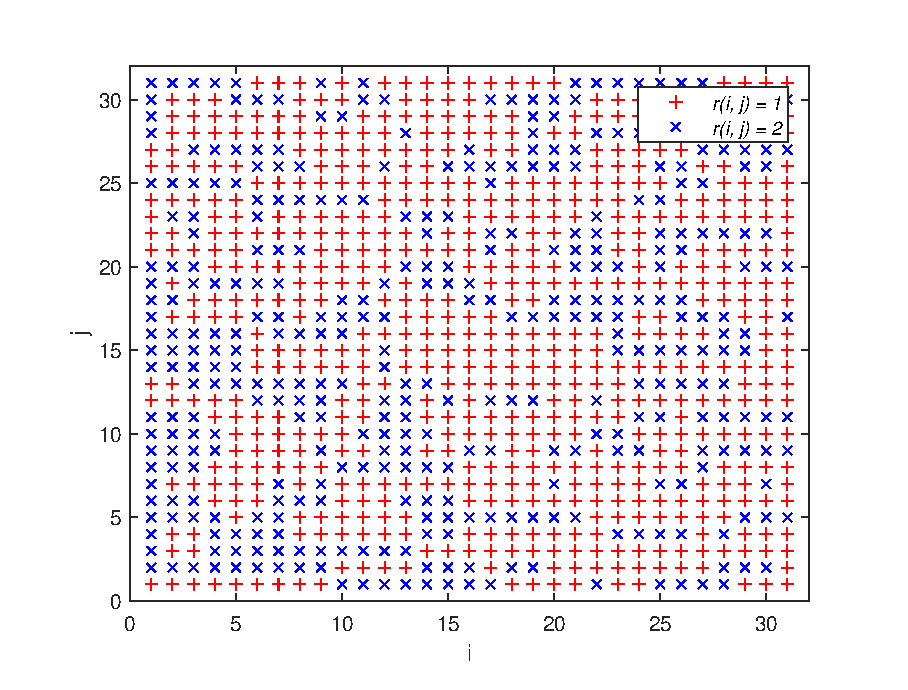
\includegraphics[scale=0.6]{./figures/2dsmc/simulations/r_eps.eps}
		\caption{系统模态变化}
		\label{fig1}
	\end{figure}
	\begin{figure}[!htb]
		\centering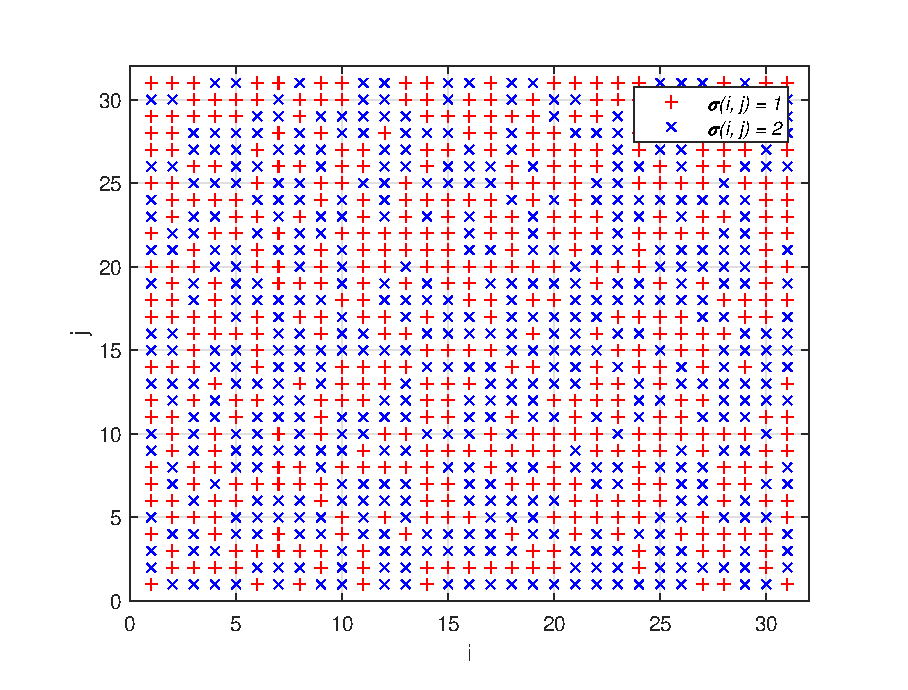
\includegraphics[scale=0.6]{./figures/2dsmc/simulations/sigma_eps.eps}\\ 
		\caption{控制器模态变化}
		\label{fig2}
	\end{figure}
	图\ref{fig1}-\ref{fig2}分别给出了一个可能的系统模态和控制器模态的演变图。通过对比,不难发现控制器的模态和系统模态是不完全匹配的。\\
	根据假设,我们设置初始条件 $X_{0}$ 和外部扰动 $w(i,j)$ 分别为
	\begin{equation*}
	\begin{aligned}
	x^{h}(0, j)&=\begin{cases}
	0.1, \quad 0\leq j \leq 10 \\
	0, \quad \ \ elsewhere
	\end{cases} \\
	x^{v}(i, 0)&=\begin{cases}
	0.1, \quad 0\leq i \leq 10 \\
	0, \quad \ \ elsewhere
	\end{cases}\\
	w(i, j)\ &=\begin{cases}
	0.2, \quad 0\leq i,j \leq 10 \\
	0, \quad \ \ elsewhere
	\end{cases}
	\end{aligned}
	\end{equation*}
	\begin{figure}[!htb]
		\centering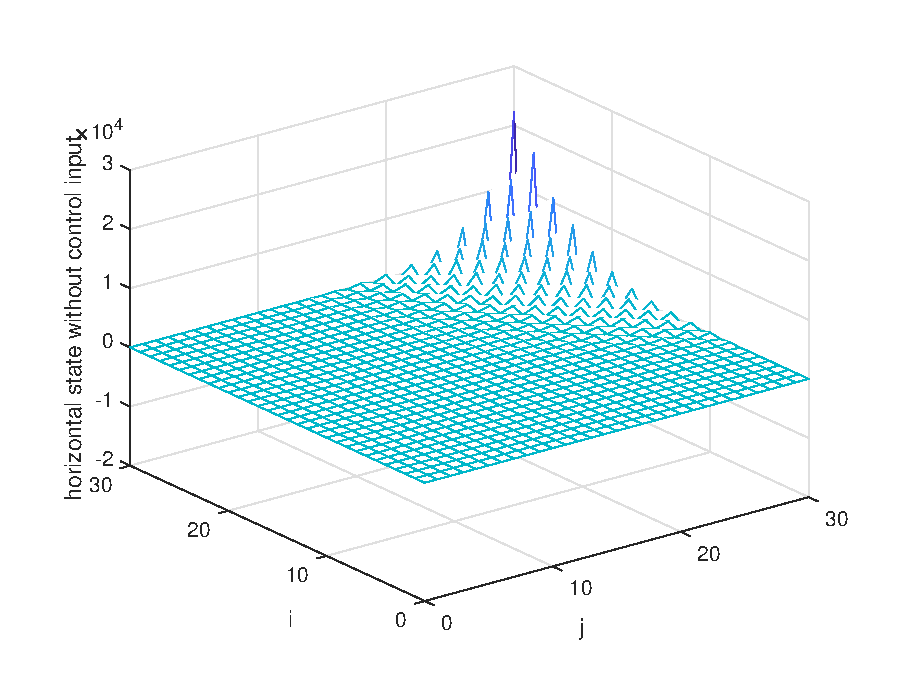
\includegraphics[scale=0.6]{./figures/2dsmc/simulations/hx-no-controll-input.eps}
		\caption{  $u(i,j)=0$时水平方向系统状态轨迹}
		\label{fig3}
	\end{figure}
	\begin{figure}[!htb]
		\centering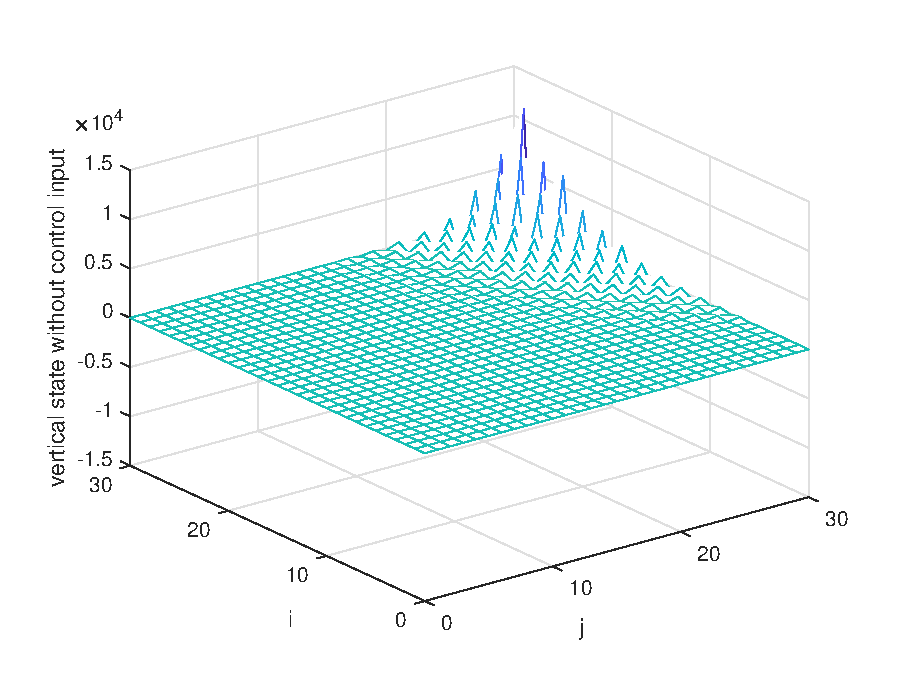
\includegraphics[scale=0.6]{./figures/2dsmc/simulations/vx-no-controll-input.eps}\\ 
		\caption{ $u(i,j)=0$时垂直方向系统状态轨迹}
		\label{fig4}
	\end{figure}
	系统 \eqref{system-equation} 在 $u(i,j) = 0$ 时系统的水平、垂直方向的系统子状态变化如图  \ref{fig3} 和\ref{fig4}。 不难看出,在不施加控制作用时,系统是不稳定的。
	然后我们按照提出的算法步骤,来进行控制器的求解。令 $\beta_{1}=0.6$ 、 $\beta_{2}=0.4$,然后求得矩阵 $G$ 为
	\begin{equation*}
	G=\begin{bmatrix}
	0.2&-0.16\\
	-0.02&-0.26
	\end{bmatrix}
	\end{equation*}
	不难验证矩阵 $GB_{k}$ 是非齐次的。参数 $\varrho_{1}$ 和 $\varrho_{2}$ 可以分别求得为 $\varrho_{1}=0.3$, $\varrho_{2}=0.6872$。 通过求解最优化问题 \eqref{optimization-problem},我们求得控制器增益为\\
	
	模态1:
	\begin{equation*}
	K_{1}=\begin{bmatrix}
	4.4147  & -4.3512\\
	-0.6827 &  -2.1886
	\end{bmatrix}
	\end{equation*}
	
	模态2:
	\begin{equation*}
	K_{2} = 	\begin{bmatrix}
	4.3706  & -3.8453 \\
	-0.6826 &  -2.3252 \\
	\end{bmatrix}
	\end{equation*}
	并且,对应的最优$H_{\infty}$ 性能为 $\gamma^{*}=0.3164$。
	\begin{figure}[!htb]
		\centering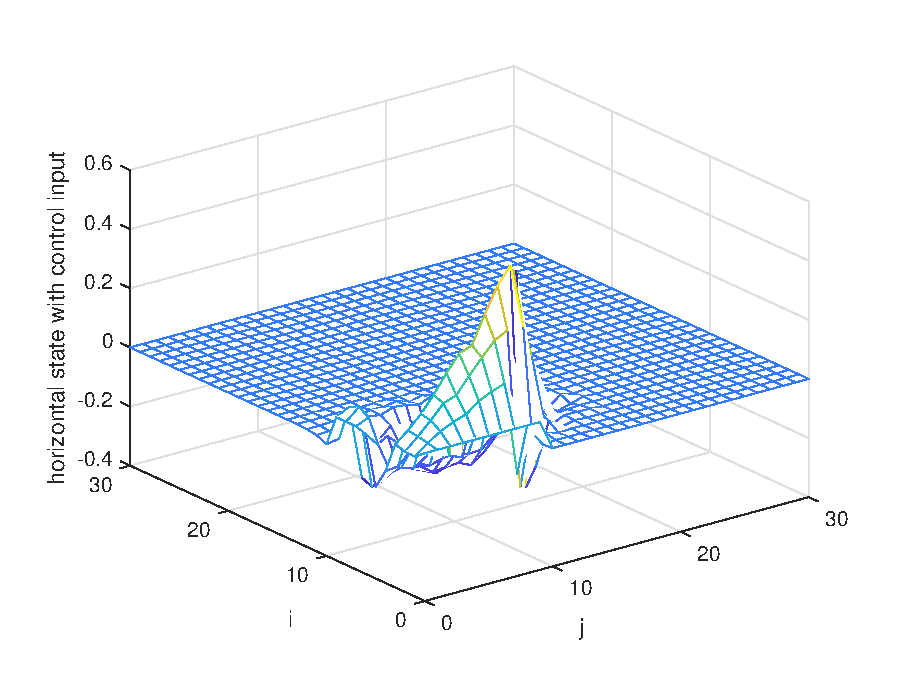
\includegraphics[scale=0.6]{./figures/2dsmc/simulations/h-state-with-force.eps}
		\caption{滑模控制器作用下的水平方向系统状态轨迹}
		\label{fig5}
	\end{figure}
	\begin{figure}[!htb]
		\centering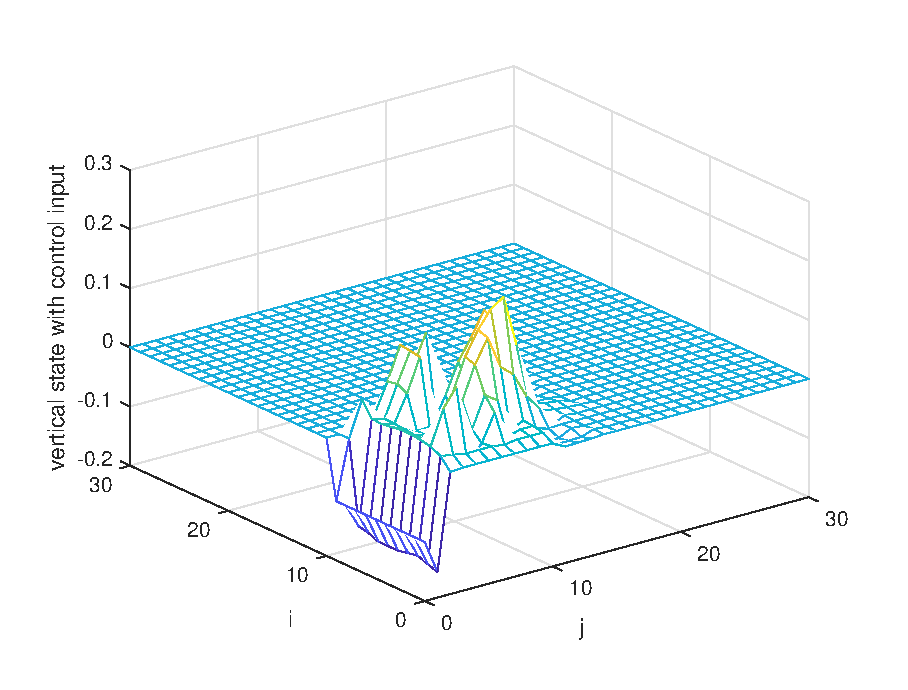
\includegraphics[scale=0.6]{./figures/2dsmc/simulations/v-state-with-force_eps.eps}\\ 
		\caption{滑模控制器作用下的垂直方向系统状态轨迹}
		\label{fig6}
	\end{figure}
	\\闭环控制系统 \eqref{closed-loop-system-equation} 在异步滑模控制器作用下的水平方向系统状态、垂直方向系统状态分别描绘在图\ref{fig5}-\ref{fig6}。显然,当施加了异步滑模控制器之后,系统状态收敛,因此系统是稳定的。可以通过条件 \eqref{siding-surface-equation} 和\eqref{smc-law}来分别求得滑模面和异步滑模控制率。 然后,图\ref{fig7}-\ref{fig10}分别给出了水平方向、垂直方向的滑模面,水平方向、垂直方向的控制输入图。 综合仿真结果,可以表明我们的异步滑模控制器是有效的。
	\begin{figure}[!htb]
		\centering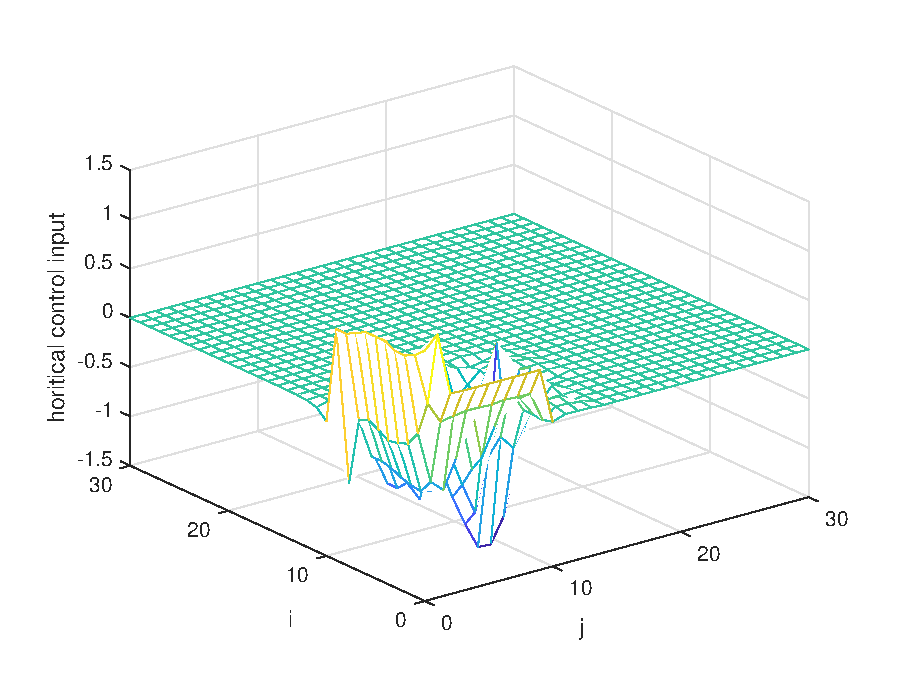
\includegraphics[scale=0.6]{./figures/2dsmc/simulations/h-control-input_eps.eps}
		\caption{水平方向异步滑模控制输入 $u^{h}(i,j)$}
		\label{fig7}
	\end{figure}
	\begin{figure}[!htb]
		\centering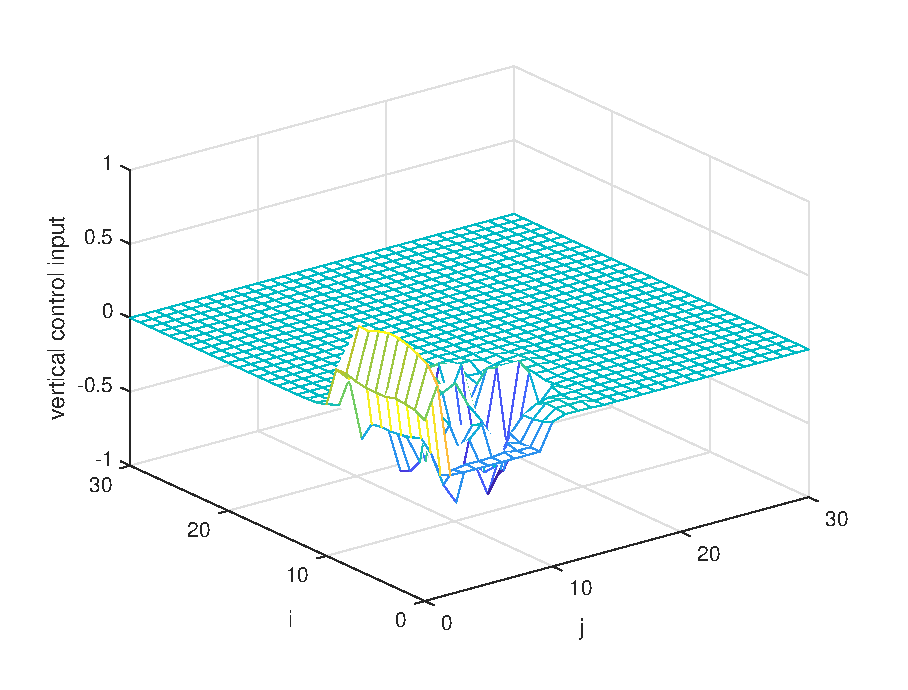
\includegraphics[scale=0.6]{./figures/2dsmc/simulations/v-controll-input_eps.eps}\\ 
		\caption{垂直方向滑模控制输入 $u^{v}(i,j)$}
		\label{fig8}
	\end{figure}
	
	\begin{figure}[!htb]
		\centering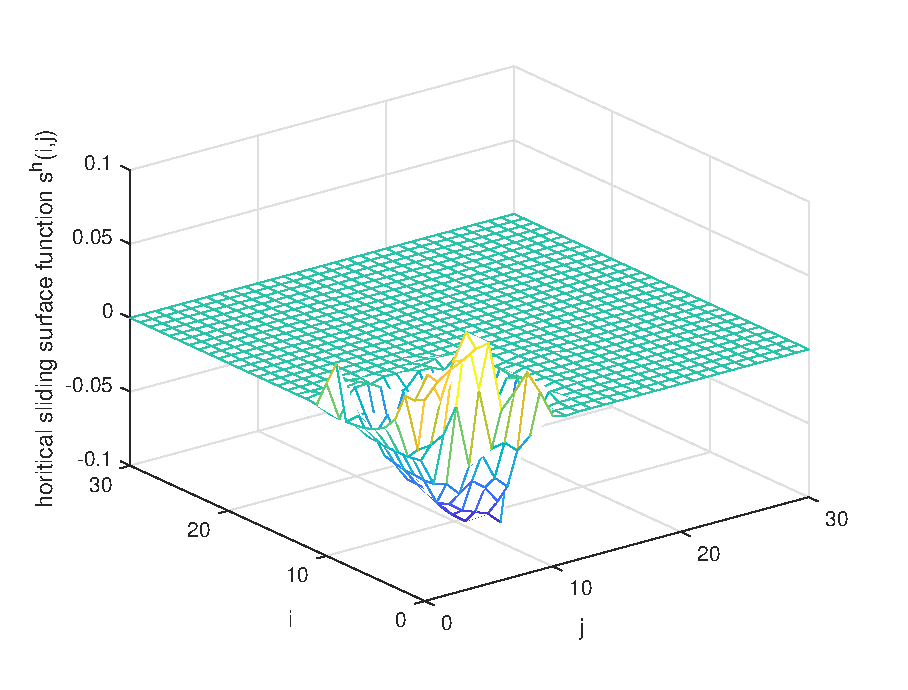
\includegraphics[scale=0.6]{./figures/2dsmc/simulations/hs_eps.eps}
		\caption{水平方向滑模面 $s^{h}(i,j)$}
		\label{fig9}
	\end{figure}
	\begin{figure}[!htb]
		\centering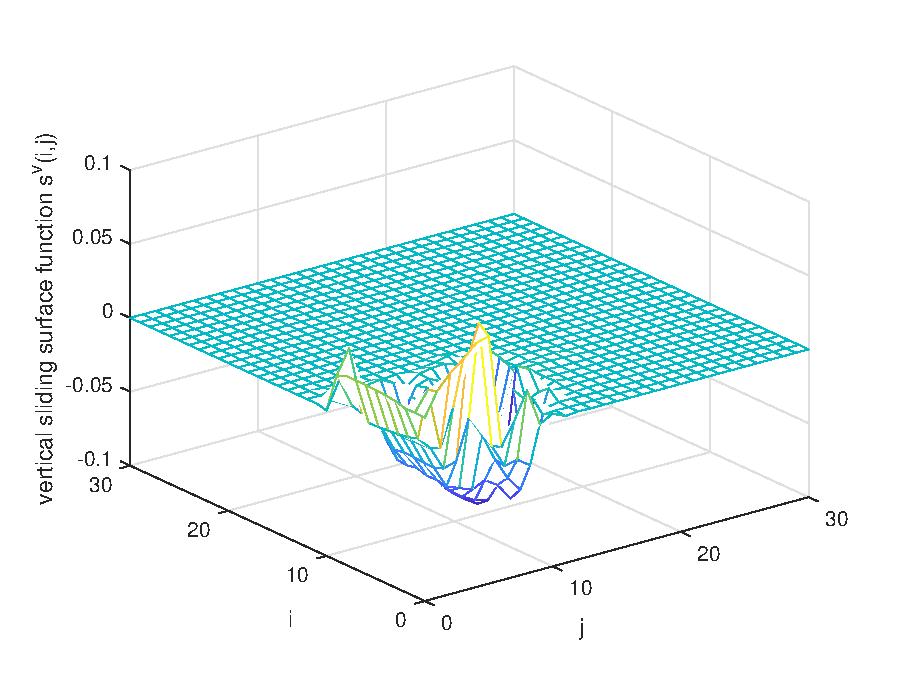
\includegraphics[scale=0.6]{./figures/2dsmc/simulations/vs_eps.eps}\\ 
		\caption{垂直方向滑模面 $s^{v}(i,j)$}
		\label{fig10}
	\end{figure}

\section{小结} \label{conclusion} 	
	本章我们研究了Roesser模型下的二维Markov跳变系统的异步滑模控制问题。考虑到控制器模态同系统模态的不匹配问题,我们基于隐Markov模型设计了异步滑模控制器。借助Lyapunov泛函方法,我们研究了系统的稳定性及其$H_{\infty}$性能,以及系统状态到滑模面的可达性问题。给出了能够使得系统稳定,且满足一定$H_{\infty}$的充分条件,同时,该条件可以保证系统状态到滑模面的可达性。最后,我们通过一个例子来验证了提出方法的有效性。
	